\clearpage
\section{System Identification}
\label{sec:systemIdentification}
A grey box model time domain approach was used to identify the unknown free parameters of the motor. This is because we know beforehand that the motor acts as a second order system whose output given a step input is:

\begin{equation}
	\frac{q}{s(\frac{s^2}{\omega^2_n} + \frac{2\xi}{\omega_n}s + 1)}
\end{equation}

The parameters to be identified include:
\begin{itemize}
	\item The natural frequency, $\omega _n$
    \item The damping factor, $\xi$
\end{itemize}
These parameters can be calculated from the estimates of the settling time and the overshoot.
\newline
\subsection{Overshoot}
\label{sec:overshoot}
The overshoot is the maximum value reached by the time evolution of the output with respect to the steady state calue. It is calculated as follows:
\begin{equation}
 O = \frac{|\chi _{max} - \chi (\infty )|}{|\chi (0) - \chi (\infty )|}
\end{equation}

Where:
\begin{itemize}
	\item $\chi (0)$ is the initial value
    \item $\chi _{max}$ is the maximum value reached
    \item $\chi (\infty )$ is the steady state value
\end{itemize}

Overshoots for the different power values were estimated and plotted as below.

\begin{figure}[H]
\centering
	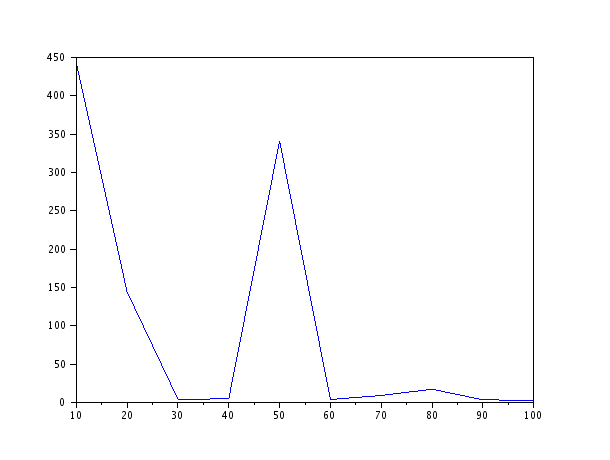
\includegraphics[scale=0.5]{images/_power_vs_overshoot.png} \\
    \caption{A graph showing the changes in the overshoot(y-axis) with power(x-axis)}
\end{figure}


\subsection{Settling Time, $T _s$}
The settling time, $T _s$ is assumed to be the time the output reaches within a given $\alpha$ value of the steady state value, $\chi (\infty )$ and forever stays there.
\newline
$\alpha=0.01 $ was used. It was calculated as,
\begin{equation}
st\_est = t(index) - StepValue/2; 
\end{equation}
where,
\begin{itemize}
	\item $t(index)$ is the time when the output first reaches the interval.
    \item $StepValue$ is the interval between two consecutive outputs.
\end{itemize}

\begin{figure}[H]
\centering
	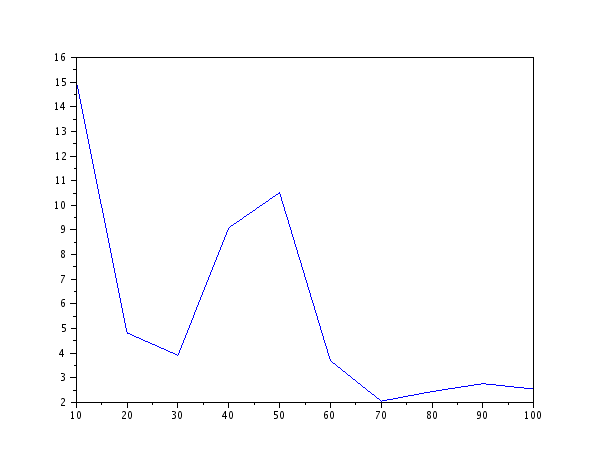
\includegraphics[scale=0.5]{images/_power_vs_st.png} \\
    \caption{A graph showing the changes in the settling time estimates(y-axis) with power(x-axis)}
\end{figure}

\subsection{Damping Factor, $\xi$}
\label{sec:dampingFactor}
The damping factor, $\xi$ estimate is calculated as:
\begin{equation}
 \xi = \sqrt{\frac {\log (ov)^2}{\pi + \log (ov)^2}}
\end{equation}
Where  $ov$ is the overshoot.


\begin{figure}[H]
\centering
	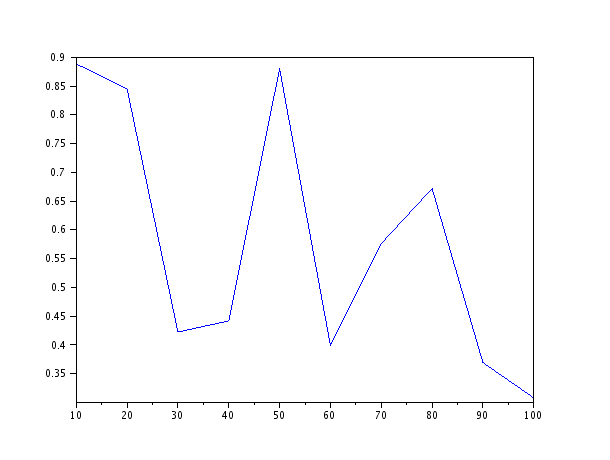
\includegraphics[scale=0.5]{images/_power_vs_xi.png} \\
    \caption{Changes in the $\xi$ estimate value(y-axis) with power(x-axis)}
\end{figure}

\subsection{Natural Frequency, $\omega _n$}
\label{sec:natFreq}
The natural frequency, $\omega _n$ is calculated as,
\begin{equation}
 \omega _n = \frac{\log (\alpha ) - \log (nb)}{-\xi st}
\end{equation}
where,
\begin{itemize}
	\item
     \begin{equation} 
		nb = \frac{1}{\sqrt{1 - \xi ^2}} 
	 \end{equation}
	\item $st$ is the settling time estimate.
\end{itemize}

\begin{figure}[H]
\centering
	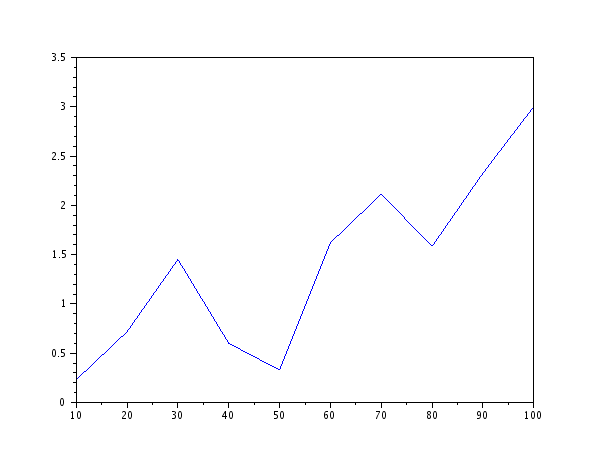
\includegraphics[scale=0.5]{images/_power_vs_omega.png} \\
    \caption{Changes in the $\omega _n$ estimate value(y-axis) with power(x-axis)}
\end{figure}

An estimate of $\omega$, $\xi$ settling time and the overshoot for each power value is presented below.
\newline 
\begin{figure}[H]
\begin{center}
	\begin{tabular}{ |l | l | l | l| l | }
		\hline
		Power & $\xi$ & $\omega _n$ & set time(s) & Overshoot \\
        \hline
        10 & 0.888824 & 0.230329 & 15.055 & 442.951331 \\
        \hline
        20 & 0.845369 & 0.718232 & 4.825 & 144.275678 \\
        \hline
        30 & 0.422576 & 1.451258 & 3.915 & 4.326551 \\
        \hline
        40 & 0.441914 & 0.600584 & 9.085 & 4.70033 \\
        \hline
        50 & 0.88039 & 0.329319 & 10.515 & 341.038526 \\
        \hline
        60 & 0.399064 & 1.620381 & 3.695 & 3.924681 \\
        \hline
        70 & 0.576415 & 2.114344 & 2.055 & 9.171027 \\
        \hline
        80 & 0.672154 & 1.583978 & 2.445 & 17.321917 \\
        \hline
        90 & 0.369445 & 2.325918 & 2.765 & 3.46885 \\
        \hline
        100 & 0.308024 & 3.000851 & 2.545 & 2.765275 \\
        \hline
        
	\end{tabular}
    
\end{center}
\caption{A table showing the values for $\xi$, $\omega _n$, settling time and overshoot for the different power values}
 \end{figure}

\subsection{Parameter Approximation}
\label{sec:parApprox}
A simple average is chosen to compute the values of $\xi$ and $\omega _n$ and they are therefore computed as follows:

\begin{equation} 
    \xi = \frac{1}{N}\sum _{i=1}^{N}\xi _{i,est} 
\end{equation}

\begin{equation} 
    \omega _n = \frac{1}{N}\sum _{i=1}^{N}\omega _{i,est} 
\end{equation}

The following values were arrived at:
\begin{itemize}
 	\item $\xi=0.5804175$
    \item $\omega _n=1.3975257$
\end{itemize}

























